\documentclass[12pt,]{article}
\usepackage{lmodern}
\usepackage{amssymb,amsmath}
\usepackage{ifxetex,ifluatex}
\usepackage{fixltx2e} % provides \textsubscript
\ifnum 0\ifxetex 1\fi\ifluatex 1\fi=0 % if pdftex
  \usepackage[T1]{fontenc}
  \usepackage[utf8]{inputenc}
\else % if luatex or xelatex
  \ifxetex
    \usepackage{mathspec}
  \else
    \usepackage{fontspec}
  \fi
  \defaultfontfeatures{Ligatures=TeX,Scale=MatchLowercase}
\fi
% use upquote if available, for straight quotes in verbatim environments
\IfFileExists{upquote.sty}{\usepackage{upquote}}{}
% use microtype if available
\IfFileExists{microtype.sty}{%
\usepackage{microtype}
\UseMicrotypeSet[protrusion]{basicmath} % disable protrusion for tt fonts
}{}
\usepackage[left=1in, right=1in, top=1in, bottom=1in, headheight=12pt, letterpaper]{geometry}
\usepackage{hyperref}
\hypersetup{unicode=true,
            pdftitle={A great title},
            pdfauthor={Author One\^{}\{1\}, Author Two\^{}1, and Author Three\^{}2},
            pdfborder={0 0 0},
            breaklinks=true}
\urlstyle{same}  % don't use monospace font for urls
\usepackage{graphicx,grffile}
\makeatletter
\def\maxwidth{\ifdim\Gin@nat@width>\linewidth\linewidth\else\Gin@nat@width\fi}
\def\maxheight{\ifdim\Gin@nat@height>\textheight\textheight\else\Gin@nat@height\fi}
\makeatother
% Scale images if necessary, so that they will not overflow the page
% margins by default, and it is still possible to overwrite the defaults
% using explicit options in \includegraphics[width, height, ...]{}
\setkeys{Gin}{width=\maxwidth,height=\maxheight,keepaspectratio}
\IfFileExists{parskip.sty}{%
\usepackage{parskip}
}{% else
\setlength{\parindent}{0pt}
\setlength{\parskip}{6pt plus 2pt minus 1pt}
}
\setlength{\emergencystretch}{3em}  % prevent overfull lines
\providecommand{\tightlist}{%
  \setlength{\itemsep}{0pt}\setlength{\parskip}{0pt}}
\setcounter{secnumdepth}{0}
% Redefines (sub)paragraphs to behave more like sections
\ifx\paragraph\undefined\else
\let\oldparagraph\paragraph
\renewcommand{\paragraph}[1]{\oldparagraph{#1}\mbox{}}
\fi
\ifx\subparagraph\undefined\else
\let\oldsubparagraph\subparagraph
\renewcommand{\subparagraph}[1]{\oldsubparagraph{#1}\mbox{}}
\fi

%%% Use protect on footnotes to avoid problems with footnotes in titles
\let\rmarkdownfootnote\footnote%
\def\footnote{\protect\rmarkdownfootnote}

%%% Change title format to be more compact
\usepackage{titling}

% Create subtitle command for use in maketitle
\newcommand{\subtitle}[1]{
  \posttitle{
    \begin{center}\large#1\end{center}
    }
}

\setlength{\droptitle}{-2em}
  \title{A great title}
  \pretitle{\vspace{\droptitle}\centering\huge}
  \posttitle{\par}
  \author{Author One\(^{1}\), Author Two\(^1\), and Author Three\(^2\)}
  \preauthor{\centering\large\emph}
  \postauthor{\par}
  \date{}
  \predate{}\postdate{}

\usepackage{mathptmx}
\usepackage{bm}
\usepackage{setspace}
\usepackage{booktabs}
\doublespacing
\usepackage{lineno}
\linenumbers

\begin{document}
\maketitle

\setlength{\abovedisplayskip}{0pt}\raggedright

\(^1\) Department of Wildland Resources and the Ecology Center, Utah
State University, Logan, UT, United States

\(^2\) Some other affiliation

\hypertarget{abstract}{%
\section{Abstract}\label{abstract}}

This is an R Markdown manuscript template. See link for more information
on R Markdown tips and tricks

\emph{Keywords: R Markdown, manuscripts, etc.}

\hypertarget{introduction}{%
\section{Introduction}\label{introduction}}

Put intro here. And make sure to cite good papers (Teller et al. 2016,
Tredennick et al. 2017). Also cite papers in text, like I am sure Teller
et al. (2016) did at some point.

\hypertarget{methods}{%
\section{Methods}\label{methods}}

What did you do?

\hypertarget{study-site-subsection}{%
\subsection{Study site (subsection)}\label{study-site-subsection}}

\hypertarget{statistical-analysis-subsection}{%
\subsection{Statistical analysis
(subsection)}\label{statistical-analysis-subsection}}

\hypertarget{results}{%
\section{Results}\label{results}}

Wow, great results (Figure 1, Table 1).

\begin{figure}
\centering
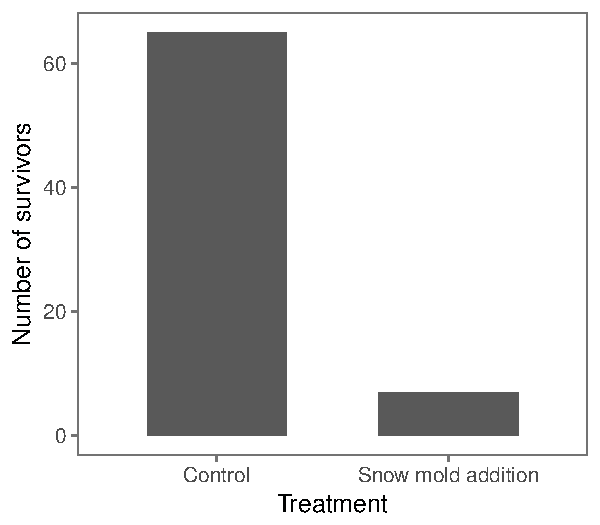
\includegraphics[width=\textwidth,height=2in]{../figures/lab_results_fig.pdf}
\caption{Whoa, a bar graph with a caption.}
\end{figure}

\hypertarget{discussion}{%
\section{Discussion}\label{discussion}}

Something profound.

\hypertarget{references}{%
\section*{References}\label{references}}
\addcontentsline{toc}{section}{References}

\hypertarget{refs}{}
\leavevmode\hypertarget{ref-Teller2016}{}%
Teller, B. J., P. B. Adler, C. B. Edwards, G. Hooker, R. E. Snyder, and
S. P. Ellner. 2016. Linking demography with drivers: climate and
competition. Methods in Ecology and Evolution 7:171--183.

\leavevmode\hypertarget{ref-Tredennick2017a}{}%
Tredennick, A. T., M. B. Hooten, and P. B. Adler. 2017. Do we need
demographic data to forecast plant population dynamics? Methods in
Ecology and Evolution 8:541--551.


\end{document}
